% This is samplepaper.tex, a sample chapter demonstrating the
% LLNCS macro package for Springer Computer Science proceedings;
% Version 2.20 of 2017/10/04
%
\documentclass[runningheads]{llncs}
\usepackage[hyphens]{url}
\usepackage{graphicx}
\usepackage{xcolor,colortbl}
\usepackage{mdframed}
\usepackage{multirow}
\usepackage{multicol}
\usepackage{comment}
\usepackage{amsmath}
\usepackage[utf8]{inputenc}
\usepackage[T1]{fontenc}
\usepackage[inline]{enumitem}
% Used for displaying a sample figure. If possible, figure files should
% be included in EPS format.
%
% If you use the hyperref package, please uncomment the following line
% to display URLs in blue roman font according to Springer's eBook style:

\mdfdefinestyle{RQFrame}{
 outerlinewidth=0pt,
 skipabove=0pt,
 skipbelow=0pt,
 innertopmargin=6pt,
 innerbottommargin=0pt,
 linewidth=0pt,
 topline=false,
 rightline=false,
 leftline=false,
 innerrightmargin=4pt,
 innerleftmargin=4pt}

\newcounter{RQCounter}
\newcommand{\RQ}[2]{
\refstepcounter{RQCounter} \label{#1}
\begin{mdframed}[style=RQFrame]\noindent
    \textbf{RQ}$_{\arabic{RQCounter}}$.~\emph{#2}
\end{mdframed}
}
\newcommand{\hr}[1]{\textbf{RQ}$_{\ref{#1}}$}
\definecolor{Gray}{gray}{0.9}
\newcommand{\mysubsec}[1]{\smallskip \emph{\textbf{#1.}}}



\usepackage{hyperref}
\renewcommand\UrlFont{\color{blue}\rmfamily}

\begin{document}

%
\title{Developing and evaluating a hackathon approach to foster cybersecurity learning}
%
%\titlerunning{Abbreviated paper title}
% If the paper title is too long for the running head, you can set
% an abbreviated paper title here
%
\titlerunning{Developing and evaluating a hackathon approach to foster cybersecurity learning}

%\author{Abasi-amefon O. Affia \and Alexander Nolte \and Raimundas Matulevi\v{c}ius }
%\institute{Institute of Computer Science, \\ University of Tartu, Tartu, Estonia,\\
%\email{amefon.affia@ut.ee, alexander.nolte@ut.ee, rma@ut.ee}
%}
%
\authorrunning{}
%\authorrunning{Affia et al.}
%
\maketitle              % typeset the header of the contribution
%
\begin{abstract}
Security research and development towards securing information systems% especially the internet of things (IoT) 
is on the increase due to the increased usage and possible applications. As such, there is a great need to train, spread awareness, and encourage people to explore the security of these information systems, and for that, hackathons might be a good approach. This paper describes the design and evaluation of a hackathon approach that fosters cybersecurity security. Evaluating our approach we found that ....
% findings
\keywords{Hackathons  \and Security \and Learning \and Action Research.}
\end{abstract}
%
%
% Hackathons are increasingly popular across different domains in recent years including the security domain. 

\section{Introduction}
Technological advancements have led to the ubiquitous availability of data and continue to shape digital innovation \cite{davenport2013analytics}. Industry experts predict there will be 6 billion internet users by 2022 \cite{cybersecventures2019} and nearly 26 billion connected devices by 2020 \cite{hung2017gartner}. An important security measure for the success and growth of information systems is the level of knowledge and awareness among human users which build these systems and/or are a part of its network \cite{mahmoud2015internet}. It has been noted that there is a need for technical professionals important to guarantee for the rapid development of the Internet of Things even in the domain of security \cite{yu2010exploration}. 
%Education is one of the key enabling factors to achieving system security in smart industries \cite{tuptuk2018security}, 
However, there is widespread ignorance of likely threats and adversaries with end-users or administrators of these information systems. %In contribution to continuous research, development and innovation in IoT security, methods to improve cybersecurity learning as a contribution to already existing methods for IoT innovation is imperative. 
Cybercriminals are continually developing more advanced and scale able tools to access these user sensitive data. Already, more than 4.5 billion records were breached in the first half of 2018\footnote{\url{https://www.gemalto.com/press/Pages/Data-Breaches-Compromised-3-3-Billion-Records-in-First-Half-of-2018.aspx} (accessed at 11/03/2020)}. To mitigate security risks associated with information systems it is necessary to consider people, processes, objects, and data. So, securing these systems and raising awareness about how to securely use them is one of the great challenges of the coming years.  %Solving these challenges form a part of digital innovation and such innovations are as a result of collaborative processes in (interdisciplinary) teams rather than as the work of individuals\cite{steen2011benefits}.

We propose to utilize the hackathon format as a way to spreading cybersecurity knowledge to the larger population. Hackathons are time-bounded events during which participants from diverse backgrounds form teams and work on projects that are of interest to them \cite{pe2018designing}. They have seen a steep rise in popularity in recent years and have been organized in a variety of domains including corporations \cite{nolte2018you,komssi2015hackathons}, start-ups \cite{nolte2019touched,cobham2017hackathon1}, (higher) education \cite{porras2019code,kienzler2017learning}, civic engagement, \cite{lodato2016issue,henderson2015getting} and others. Among others they have been proposed as a tool for teaching to educational curricula in general \cite{abdullah2015stimulating,porras2019code,sakhumuzi2017student,nandi2016hackathons} and to train users in various concepts of cybersecurity in particular \cite{weiss2015teaching,kharchenko2016university,boopathi2015learning}. Learning has in fact been cited as one of the key motivations for participants to join hackathons \cite{porras2019code,briscoe2014digital,juell2014public}.

While learning can be considered an essential part of every hackathon prior work provides indication that what organizers want participants to learn can be different from what they actually learn or are interested in learning \cite{medina2019does}. It is thus necessarily to purposefully design hackathons to foster cybersecurity learning but it is at the same time unclear which strategies indeed foster the desired learning outcomes. Our study addresses this gap by developing and evaluating a hackathon approach that aims to foster cybersecurity learning in a hackathon. Based on prior work in the hackathon domain we proposed specific intervention to the hackathon approach thus aiming to answer the following two related research questions:

%To accelerate the development of new service ideas and prototypes, innovation type contests, have become popular instruments \cite{bullinger2010innovation,hjalmarsson2012designing,soltani2014hackathon,juell2014public}. However, only a few of the service prototypes developed at innovation contests become viable digital services \cite{hjalmarsson2014beyond}. 
%However, few studies have addressed perceived learning in security based hackathons. 

\RQ{RQ1}{How can different interventions at a hackathon influence learning?}
\RQ{RQ2}{How can these interventions be improved?}

To answer these questions, we conducted an action research study of three teams at a cybersecurity hackathon. The methods and processes to stimulate learning were provided as interventions introduced during the hackathon process. We observed all teams and participants during the hackathon at set intervals during its early, mid, and later phases, administered surveys and conducted interviews at the end of the hackathon event.

Our results indicate ....

\section{Background}
In the following section we will discuss our work in the context of prior work on hackathons in cybersecurity (section \ref{Sec:relatedworks}) before focusing on learning in particular (section \ref{Sec:designaspects}).

\subsection{Related Works}\label{Sec:relatedworks}
Hackathons are intense, uninterrupted and \textit{time-bounded} events, typically of 2-5 days, during which people gather together and form \textit{collocated teams}, in attempts to complete a \textit{project} of interest \cite{nolte2018you,komssi2015hackathons}. Hackathons in the security domain have mainly been used to facilitate training and awareness in the cybersecurity community and to train future cybersecurity professionals. Research into security hackathons resulted in few reported results in studies amidst security hackathon popularity\footnote{\url{https://www.hackathon.com/theme/cybersecurity} (accessed at 11/03/2020)}, few of them have reported their findings academically. 

Kharchenko et al. \cite{kharchenko2016university}, presented a case study collection which reports on the analysis the organisation of hackathons for cybersecurity development. %The presented case study included a hackathon organised and targeted at learning cybersecurity features of embedded systems. At the hackathon, security experts gave presentations to provide cybersecurity knowledge and to discuss cybersecurity concepts. Participants were then divided into teams for a competition to solve theoretical and practical problems in different teams and results assessed by experts.
They did not report on an evaluation on the design aspects that fostered cybersecurity learning and the learning objectives of the hackathon though. Similarly, the paper by Starov et al. \cite{starov2015hacking}, reports on a hackathon where students were provided comprehensive knowledge in a special course, then participated in an idea generation and prototype development training. %These equipped the students to develop projects and participate in competitions.
The emphasis of this study was on start-up development and establishing communication between university and industry. The study did not show any evaluation of learning objectives or design aspects to foster learning. Finally, Foley et al. \cite{foley2018science} discuss findings from a case study on a science hackathon where researchers, using transverse use-cases on shared CPS testbed platforms, explain ongoing research in securing cyber-physical systems (CPS), learn and teach each other about the technology, and develop prototypes. %Learning experiences of the participants, as well as the communicative ability of this hackathon about cybersecurity, were discussed. Although the study examines learning experiences, 
The paper does not report on an evaluation of the design aspects that foster awareness and cybersecurity learning though.

Our work is thus different from prior studies on cybersecurity learning at hackathons because we aim to develop and evaluate specific interventions and identify means for improving them.

\subsection{Hackathon Design aspects for Learning}\label{Sec:designaspects}
Designing hackathons that foster learning require careful planning. The design should create a learning environment suitable for learning through problem-solving \cite{case2004between}. Participants should be able to gain sufficient knowledge about cybersecurity to explore and contribute to the development of security solutions within the tight time constraints of the hackathon. Thus, certain design decisions are essential to define the learning environment and goals \cite{kollwitz2019hack}. 

...

Part of each hackathon is for teams to generate ideas that are aligned to the theme of the event and that form the basis of the project they will work on during the event. It is thus crucial for hackathons to start with an open ideation phase \cite{bohmer2015open} where teams can express and refine ideas. %Moreover it allows teams to explore Initial ideas ... Participants then further refine their selected ideas to ensure it aligns with the theme of the hackathon and holds value in solving real security issues. In Pe-Than et al. \cite{pe2018designing}, the study observed that a reasonably extensive idea preparation characterises winning teams. Here, participants learn through discussions on the challenge subject domain, and by the development of an idea based on an understanding of the challenge. 
In highlighting the focus of the hackathon, decisions to drive the theme and encourage the participants to learn by accomplishing the challenge output are essential. Having a security talk at the hackathon provides context to the goal of the hackathon. It allows participants to discuss the basics of security within the current advances in information systems with its existing security issues. 
Although participation in the hackathon is voluntary, specific incentives can encourage %the value of cooperation and innovation within a given hackathon project and, possibly, an encouragement
individuals to participate. Competition style design features can provide these incentives that shape participation \cite{grimes2008robotics} within the time and environmental constraints. Strategic competition prizes set the goal for participants and provide the opportunity for further development of the security solution produced in the form of offering post-hackathon resources.
Other decisions include resources or inputs provided to participants during the hackathon that can encourage learning. Feedback from mentors offer experience and insights to guide projects, especially in scoping, and aid problem solving by providing suggestions about alternative ways to approach a problem, given the limited time frame of the hackathon \cite{lara2016hackathons}. Mentorship also allows participants to receive learning-oriented support, especially when there is a positive dynamic between participant and mentor, leading to an assumption of a role closer to that of a traditional (workplace or educational) mentor \cite{nolte2018support}.

%The typical hackathon process \cite{komssi2014hackathons} includes three stages -- pre-hackathon, hackathon, and post-hackathon phases. The pre-hackathon stage allows to better frame the problem to be solved or the hackathon event i.e. idea generation, team building. The hackathon stage (event) accelerates project ideas towards a prototype or other proof of concept, and the post-hackathon stage allows to develop a more robust product or service.

\subsection{Evaluation of Design aspects}\label{sec:blooms}
We also evaluate the effect of design aspects introduced and the learning objectives of the participants of the hackathon. We assess the learning objectives and knowledge gained by the participants using Bloom's Taxonomy, and the effect of the introduced design aspects in learning is analysed based on data collected about the hackathon event.

Bloom's Taxonomy describes levels of learning where categories of Remember, Understand, Apply, Analyze, Evaluate, and Create form the cognitive learning process dimension that participates in knowledge dimensions \cite{bloom1956taxonomy,krathwohl2009taxonomy}.
\begin{itemize}
    \item \textbf{Remember} includes the retrieving, recognizing, and recalling relevant knowledge provided by the design aspects from memory.
    \item \textbf{Understand} constructs meaning from oral, written, and graphic messages through interpreting, exemplifying, classifying, summarizing, inferring, comparing, and explaining.
    \item \textbf{Apply} uses a given procedure through executing or implementing.
    \item \textbf{Analyze} separates knowledge or concepts into constituent parts, determining how the parts relate to one another and an overall purpose.
    \item \textbf{Evaluate} makes judgments based on criteria and standards through checking and critiquing.
    \item \textbf{Create} puts elements together to form a new pattern or structure.
\end{itemize}
In studies, the taxonomy has been used, especially in computer science fields, to assess learning outcomes and objectives that formulate how an educative process \cite{starr2008bloom,thompson2008bloom} improves students knowledge. Using bloom's, we can discern if the participants are familiar with security concepts presented at the hackathon, and can form relationships between the essential elements of security to develop a security idea. We can also discern how this knowledge was used as a baseline to carry out the intended project and, as a result, create a security prototype.

As studies do not specify which design aspects introduced in the hackathon serve to encourage learning, the connection between the levels of learning and the introduced design aspects will give us insight into what design aspects were instrumental to learning. This insight will enable us to build on such design aspects in the future, to advance security awareness and reduce the cybersecurity knowledge and skill gap.

%The taxonomy to analyse the assessable learning outcomes of each introduced design aspect. We can discern if the participants are familiar with basic security concepts, can form relationships between the essential elements of security, and use this knowledge as a baseline to develop a method of carrying out the intended project and, as a result, create a security prototype.

%The knowledge dimension follows Bloom's knowledge categories. These allow us to assess if the participants are familiar with basic security concepts, are able to form relationships between the basic elements of security and use this knowledge as a baseline to form a method of carrying out the intended project and as a result create a security prototype. The cognitive process dimension allow us to assess knowledge gained through each step of its process.

\section{Empirical Method}

To answer the research questions (\hr{RQ1} and \hr{RQ2}) posed, we used an action research approach
\cite{bhattacherjee2012social,kaplan1998innovation} to explore new forms of evaluating learning influence by set interventions. This approach is appropriate for this study because it provides guidelines to define actions to be introduced to a problem, to observe and study the introduction of these actions and analyse the results for future iterations. With action research, design decisions can be intentionally introduced as ``interventions" to influence learning in cybersecurity (\hr{RQ1}) and then observed to gain insights for future iterations of the hackathon (\hr{RQ2}).

\subsection{Proposed Interventions to Learning} \label{Sec:interventions}
The proposed interventions are design decisions that go into implementing the hackathon to provide learning opportunities. We discussed the hackathon design aspects that encourage learning in Section \ref{Sec:designaspects}. It is common for hackathons to use design aspects, but we propose specific ways in which we introduce interventions into the hackathon.

\textbf{Idea generation} intervention was introduced both as an ideation event before the hackathon event to focus on the building of security solutions and during the main hackathon event to kickstart building the security solution. Idea generation is also an important factor in building a team of people with shared interests, so networking and team-building opportunities were offered during the event. The learning objective from this intervention is that; \begin{enumerate*}[label=(\arabic*)]
  \item Participants should have an understanding of current security issues,
  \item Participants should be able to propose ideas based on the knowledge gained,
  \item Participants should be able to communicate the impact that the security knowledge gained has on the development of the proposed solution.
\end{enumerate*}

We also introduced the \textbf{Security Talks} intervention, where we organised the security talks to cover top security trends, especially in IoT, security risk management, and the need for security awareness. We intended that these discussions introduce participants new to the field, to security and encourage other participants to learn more about security techniques and concepts. The security talks should enable participants to produce better ideas generated with more detailed knowledge of the issues in security. To maximise this intervention, we introduced it at the ideation pre-hackathon events and sessions during the main hackathon event. The learning objective from this intervention is that;
\begin{enumerate*}[label=(\arabic*)]
  \item Participants should remember basic security concepts learnt from the security talks,
  \item Participants should be able to understand existing security issues and their impact.
\end{enumerate*}

\textbf{Mentor feedback} is another intervention introduced to the hackathon design. We organised mentor assignment during set checkpoint sessions, and by special need-based assignment -- where teams with special challenges are assigned mentors that will help resolve these challenges. At checkpoint sessions, participants can give short technical briefings or pitches about their ideas and product executions. The checkpoint sessions enabled mentors to see where certain teams required help in completing their security solutions. 
We implemented this intervention in such a way that each group received sufficient participation of mentors. The learning objective from this intervention is that;
\begin{enumerate*}[label=(\arabic*)]
  \item Participants should be able to incorporate mentor feedback to a security solution,
  \item Participant should be able to communicate the process of building the security solution as a result of knowledge gained.
\end{enumerate*}
 
Lastly, the \textbf{competition style} intervention was introduced throughout the hackathon event to set the environment. The incentives were provided for all participants and especially for winners. We decided that incentives for winners should be more strategic as opposed to mere cash incentives because they present opportunities for the continued development of winning security ideas and solutions. The learning objective from this intervention is that the participants should be able to apply the security knowledge gained to create a unique security prototype within the given time frame.

\subsection{Setting and procedure}
The main aim of the studied hackathon was to expose its participants to in cybersecurity issues, to find solutions to these recurring problems and challenges. Solutions expected to range from security awareness to security software/hardware prototypes. Figure \ref{Fig:timeline} shows the timeline of the hackathon process, including preparation and data collection activities before during and after the hackathon event.

Preparations for the hackathon event began five months before the main hackathon event. Before the main hackathon event, we held an ideation event to not only boost idea generation, but to provide security knowledge exchange, and bring people together from different fields to generate ideas that aim at tackling issues in cybersecurity. Here, we introduced the idea generation and security talk interventions. The pre-hackathon events started with a session to discuss the problems in security, followed by another session on how to communicate any generated security ideas effectively. After the first round of idea generation, we provided exercises that help participants think deeply and elaborate on these ideas. Sessions were also conducted with the help of skilled mentors, providing feedback on each proposed idea, and an opportunity to mature ideas into innovative prototypes. The participants generated a total of 17 ideas, and 11 of those ideas were developed and pitched at the ideation pre-hackathon event. 

At main hackathon event started with a short introduction by the hackathon organizers and mentors and an introduction to the domain at the first session of the security talk intervention. We then introduced idea generation intervention to enable participants to use knowledge from the security talks to develop ideas to solve issues raised and mentor feedback intervention to provide feedback on ideas generated.
Ideas were pitched to mentors and fellow participants, leading to a total of 17 ideas for further refinement where a participant presented an idea generated from the ideation pre-hackathon event. Mentors facilitated the documentation of all ideas and provided these to the participant for possible team formation. Once the idea generation sessions were completed, idea selection commenced. The number of ideas selected was due to the availability of team members to complete the security solution or availability of interested participants for the ideas. 
Team formation exercise led to a composition of team members between 5-8 participants per selected idea. Once the participants completed team formation for selected ideas, teamwork on the chosen project idea commenced, and mentors were also assigned as needed, based on issues raised during idea generation. Out of 17 ideas pitched, ten ideas were selected to form a suitable team. The mentor feedback intervention was also introduced at checkpoints during the hackathons to enable teams to provide updates on the solutions to the proposed ideas and get expert guidance and feedback concerning the solution and team progress. Another security talk session was presented on security risk management to provide the participants with more security considerations when building their solutions. 
All teams presented their solutions and prototypes at the end of the hackathon for evaluation. The hackathon provided live-streamed presentations of the solutions and prototypes to all interested community members. After evaluation, the judges selected the winners, and other teams could win different prizes.

\begin{figure*}[h]
%\vspace{-15pt}
  \centering
  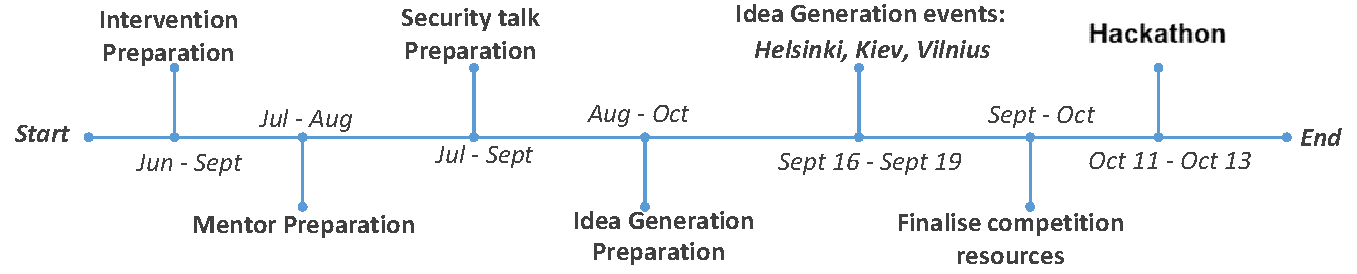
\includegraphics[width=\linewidth]{timelinehack.pdf}
  \caption{Preparation activities and data collection before, during and after the hackathon event} \label{Fig:timeline} 
 % \vspace{-20pt}
\end{figure*}

\subsection{Data collection}
We collected data for this study from different sources including planning documents, data by observation, survey, and post-hackathon interviews (c.f. Fig. \ref{Fig:timeline} for an overview of the timeline).  We will expand on how data collected from these data sources contribute to answering research question \hr{RQ2}.

Before participating in the hackathon, participants filled out an online registration form containing questions about demographic background and skills. These answers provided information relevant to aid team formation, security presentations to be delivered, and mentor compilation for the hackathon.

We moved between the teams during the hackathon event to observe the participants activities and behaviour. The observation method included monitoring at intervals and recording the responses of the participants to the interventions to influence learning in cybersecurity. Reactions such as attentiveness to security talks, positive interactions with mentors reported when discussing with a sample of participants, and perceived satisfaction of participants to the project indicated reactions to respective interventions. We also recorded other factors that may contribute to understanding the learning experience of the participants, such as teamwork, team process, or leadership influence.
We did not observe the teams throughout the hackathon as we perceived the early, mid and late phases of the hackathon to be necessary.

After the hackathon event, we supplied post-hackathon surveys to the participants. The voluntary survey covered participants motivation and preparation for the hackathon, team demographics and process, learning experience based on the interventions, and satisfaction with the experience on a 5-point Likert response scale. We collected a total of 13 responses (from 7 projects)  from the survey. Sample questions include; 
\begin{enumerate}
    \item To what extent was your decision to participate in the cybersecurity hackathon motivated by:[\textit{options list}]
    \item How did you work together on your project during the hackathon? [\textit{options list}]
    \item To what extend do you agree with the following statements about your cybersecurity learning experience at the hackathon? [\textit{[options list]: Talking with my mentors helped me learn more about cybersecurity}]
    \item Please indicate your level of agreement with the following statements related to the satisfaction with your learning experience: [\textit{options list}]
\end{enumerate}


We conducted post-hackathon interviews were then conducted with invited 6 participants to discuss the preparation process for the hackathon, the learning experiences, and the project solution worked on. The interviews are to last about 30 minutes. These post-hackathon interviews are conducted and analyzed for participants to provide a better comprehension of perceived individual and team learning experiences. A sample of questions asked during the interviews include;
\begin{enumerate}
    \item How was the hackathon from your perspective in the form of: What did you do after you arrived? How did you see the event play out? 
    \item Did you attend the pre-event? What idea did you develop? How else did you prepare for this hackathon?
    \item What were the outcomes as a result of learning? [mentors, security talks, team members, working on the project]
    \item How do you perceive the outcome of the hackathon? Were you satisfied? How did you see your teamwork? 
    \item What security issues did your project address? What security considerations did you place on the [process of creation of the product, the outcome of the project].
    \item Did you discover anything new as regards security during the hackathon? How did you discover this?
    \item What about the continuity of your project? Have you use anything learned during the hackathon already? Are you planning to use it in the future? 
    \item Do you still use any security knowledge gained during the hackathon?
\end{enumerate}


\subsection{Analysis procedure}
The analysis procedure started by analyzing interview recordings, survey results, observation notes and planning documents. The interviews and observation served as our main source of information with planning documents providing additional context. We used the surveys as additional qualitative data complementing the interview recordings.

We focused on the team as our unit of analysis, analysing how the participants in a team responded to the interventions of idea generation, security talks at the event, mentor feedback process and the competition design type. Some interesting parts of the hackathon i.e., satisfaction with the final product, team demographics i.e (size, skill diversity, familiarity, leadership) were included where they may have affected the learning experience.

Data concerning the team demographics, i.e., skill diversity was derived by calculating the similarity of perceived team skills and then revert the result by subtracting it from one.
We use data from different survey questions to assess the different interventions (see Table \ref{tab:teambinter}). This qualitative data will complement further analysis done using the observation and interview. For this mapping, we followed a strategy \cite{braun2006using} by creating and applying initial codes to the interviews based on our research questions and interesting points that could also help answer research questions. We compared the findings for each team to assess the perceived learning of one team over another.

With the data available, we can analyse the processes by which the participants encountered and worked with knowledge provided through the interventions by comparing the teams journeys.
%calculated means and standard deviations and that we use this information as part of our qualitative data analysis
%Statistically significant questions and responses from survey for learning
\begin{table}[h]
    \caption{Calculated means and standard deviations used in qualitative data analysis}
    \label{tab:teambinter}
    %\centering
    \begin{tabular}{|p{0.22\linewidth}|p{0.42\linewidth}|p{0.1\linewidth}|p{0.1\linewidth}|p{0.1\linewidth}|}\hline
	Intervention & Significant \newline Survey Question (see Appendix) &  Team A & Team B & Team C \\ \hline
	Idea generation & Q3, Q13 & $\emptyset$ & 2.25 & 2.5  \\ \hline
	Security Talks  & Q13 &  4 & 3 & 3.67   \\ \hline
	Mentor Feedback  & Q13 &  3.5 & 3 & 3.33 \\ \hline
	Competition style \newline (Final Product) & Q4, Q13, Q14, Q15 & 3.3 & 3.3 & 2.7   \\ \hline
	\multirow{8}{*}{**Team properties} & size (Q5) & 6 & 6 & 5  \\\cline{2-5}
	%& skills (Q1**, Q3) & 0.5 , 1 & 0.5,2.5 & $\emptyset$, 1  \\ \hline
	& team familiarity (Q9) & 1.125 & 4 & 1  \\ \cline{2-5}
	& motivation (Q2) & 3 & 3.92 & 2.56  \\ \cline{2-5}
	& preparation (Q4) & 1.25 & 2.75 & 1.33  \\ \cline{2-5}
	& leadership (Q7) & yes & yes & yes  \\ \cline{2-5}
	& skill diversity (Q8) & 0.6 & 0.7 & 0.4  \\ \cline{2-5}
	& collaboration process (Q10,Q11) & 3.81 & 4.56 & 4.125  \\ \cline{2-5}
	& satisfaction(Q12, Q13) & 3.9 & 2.85 & 3.35  \\ \hline
    \end{tabular}
    %*Partial evaluation as Q3 did not apply \\
    *Not interventions, but team properties that were found interesting in analysis.
\end{table}



\section{Findings}
This section outlines the journeys of each selected team, the influence of each learning intervention on each team, and the differences between teams in relation to their learning process with the introduced interventions. All variables used in this section are reflected in Table \ref{tab:teambinter}.

\subsection{Team A}
The leader of team A (P01) proposed the idea for the project in the idea generation session at the main hackathon event carried out by the team. P01 derived the idea from ``\textit{a security problem from studies''} (P01) of the hackathon and intended to create tool for enterprises to visualize security aspects. P01 formed a 6-member team with skill diversity rated at (\textit{0.6}) and team familiarity rated at ($m = 1.125$). \textit{``Ideation continued during the hackathon because the idea was not properly prepared''} (P01), and completed after discussions within the team and mentor feedback. The idea was refined to ``\textit{be targeted at company risk management team to help visualise and communicate security risk scenarios to upper management}''.

At the security talk sessions, participants from team A reported cybersecurity learning gains from the talks ($m = 4$) and showed an understanding of the security domain in moving forward with the project. P01 highlighted on the  \textit{``educating experience about risk management and what is missing in the cybersecurity field}'' presented at the security talks.

The creation of the final product within the constraints of the competition style allowed the team to work together in creating unique solutions. P01 highlights that there was ``\textit{support by experienced team members to complete tasks}'' for the project. The team leader (P01) fostered learning within the team \textit{``holding everything together, monitoring and identifying the needs of each team members for completing tasks''}. P01 described how teamwork grew and how ``\textit{everybody was eager to work and contribute in any way they could}''; ``\textit{some team members had no prior experience to security, but they tried to learn and contribute}'' (P01). P01 thus reported that the team members ``\textit{went definitely beyond their current skills}''. The team leader (P01) was involved in  \textit{``monitoring and identifying the needs of each team members for completing tasks''}, and mentors supported these responsibilities were necessary to adjust scoping of the project. At checkpoints in the hackathon event, the team leader P01, presented updates to the mentors about the project progress, getting feedback from mentors about moving forward to the prototype stage. Talking and interacting with mentors was reported to help the team learn more about cybersecurity ($m = 3.5$).

At the end of the hackathon event, team A presented the security prototype to judges for evaluation. Although team A did not win a prize at the competition, team A participants reported, a moderate learning experience from building the final product ($m = 3.3$) and an agreement on the satisfaction level from the event ($m = 3.9$), with individual comments about the \textit{``great event setup and mentoring''} (P01) and how \textit{``nicely organized''} (P02) the event was. However, P01 expressed that there will be no continuation in the project because it was \textit{``not quite sure, the market value for this type of project''} (P01), having less intent to continue with the project as opposed to another team member P02.


\subsection{Team B}
The leader of team B (P03) presented an idea developed at the pre-hackathon event. P03 highlights that attending the ideation event provided \textit{``a lot of support to [my] idea''}. The idea developed was to \textit{``make data security more desirable for startups and give them a badge''} (P03), thereby tackling the security awareness in startups issue. P03 presented the idea during the idea pitching session of the hackathon event and a little feedback provided by mentors. After ideation, P03 reports that team formation was easy. This is because P03 \textit{``was familiar with most of the team because [we] studied together at the university''}($m = 4$). P03 formed a 6-member team with skill diversity rated at (\textit{0.7}).

At the security talk sessions, P04 explained that the security talks at the hackathon event were instrumental as the team \textit{``tried to gather all sorts of information on how to secure systems and gained knowledge''}. Participants from team B reported security gains from the talks ($m = 3$). Team B participants report learning experiences from the mentor feedback ($m = 3$) as the checkpoints provided \textit{``an opportunity for [us] to explain our work progress''} (P04). Between checkpoints, P04 reported that \textit{``different mentors visited multiple times''}, and that the mentors  \textit{``visited to guide completing tasks''} (P04). P03 reports that mentors specifically provided feedback on the scoping of the project, and refinement of project content to define the life-cycle of different startups and the security implementations needed for each stage of the life-cycle as well as the business aspects.

In the creation of the final product, the team perceived their collaboration process to be efficient ($m = 4.56$). P03 mentioned that a \textit{``blackboard equipment for documenting the team's process and ideas, allowing [us] to see the big picture''}, thereby aiding collaboration between members of the team and between the team and mentors. 
The competition style of the hackathon, team B participants, reported learning experience($m = 3.3$) from accomplishing the task of building security content for the prototype.

Towards the end of the hackathon event, Team B pitched their project and presented the prototype for evaluation. Team B won a prize for a unique product developed and its perceived usefulness to the security community. Interestingly, there was a moderate satisfaction with the outcome of the project ($m = 2.9$). P03 raised an issue with a team member leaving the team unexpectedly halfway through the hackathon with the resources already gathered by the team. Continuation of the project following the competition style intervention was encouraged by the incentive prize awarded to the team project. Although P03 reported that the team intends to continue with the project, we learned from both P03 and P04 that the provided incentive might not be useful to its continuation.


\subsection{Team C}
The team lead (P05) pitched an idea during the idea generation session of the hackathon event. Although P05 attended the ideation pre-hackathon event, the idea pitched at the main hackathon event was not prepared during the pre-hackathon event. P05 pitched the idea to \textit{``create a binary betting platform for smart contracts''} on a blockchain platform. However, mentors provided feedback that the presented idea did not readily give a solution to current security issues and asked P05 to think more of the security solution. P05 formed a 5-member team with skill diversity rated at ($\textit{0.4}$), and constituting mainly of developers interested in developing a blockchain-based solution.

Once team formation was complete, the participants in team C continued idea refinement with the mentor feedback. P06 stated that the initial idea \textit{``didn't seem like a good idea for a security hackathon, so [we] needed to connect it to a security topic''}. Thus, a new idea was formed based on blockchain, where the team decided on \textit{``an availability insurance smart contract for service providers''} (P06). During checkpoint sessions, the team leader (P05) provided progress reports on development to the mentors, who contributed as much feedback as possible on enhancing the proposed security prototype. The participants of team C report learning experience from the provided mentor feedback ($m = 3.33$). Although were no individual reports from the participants of team C about learning experiences from the security talk sessions, surveys responses from team C participants report learning gains from the security talk intervention ($m = 3.67$).

The participants in team C report learning experience ($m = 3.3$) by researching the security aspects of the prototype. The team perceived their collaboration process to be efficient ($m = 4.25$). P06 highlighted that this was due to the team's high interest in development using blockchain. Towards the end of the event, Team C pitched the final prototype for evaluation. After evaluation, Team C did not win a prize at the event and reported moderate satisfaction with the outcome of the project ($m = 2.85$). P06 mentioned that the moderate outcome might be due to the difficulty faced in ideation. There were no intentions of the participants to continue with the project idea.


\subsection{Team Comparison} \label{teamcomparison}
In this section, we use bloom's taxonomy to compare the learning levels between the team's A, B and C with the knowledge of the team's activity, team's learning experience, and the learning objectives by introducing the interventions (see section \ref{Sec:interventions}). In Table \ref{tab:learningoutcomesbloom}, we summarise the learning objectives with their respective bloom's process categories, as discussed in Section \ref{sec:blooms}.
 \begin{table}[h]
    \centering
    \caption{Learning objectives to blooms process category}
    \label{tab:learningoutcomesbloom}
    \begin{tabular}{|p{0.83\linewidth}|p{0.14\linewidth}|} \hline
    Learning objectives (\textit{IG -- Idea Generation, ST -- Security Talks, MF -- Mentor Feedback, CS -- Competition Style}) & Process \newline category\\ \hline
    ($IG1$) Participants should have an understanding of current security issues & Understand \\ \hline
    ($IG2$) Participants should be able to propose ideas based on the knowledge gained, to address these security problems & Apply\\ \hline
    ($IG3$) Participants should be able to communicate the impact that the security knowledge gained has on the development of the proposed solution & Analyse \\ \hline
    ($ST1$) Participants should remember basic security concepts learnt from the security talks & Remember, \newline Understand \\ \hline
    ($ST2$) Participants should be able to understand existing security issues and its impact & Understand \\ \hline
    ($MF1$) Participants should be able to incorporate mentor feedback to security solution & Apply \\ \hline
    ($MF2$) Participant should be able to communicate the process of building the security solution as a result of knowledge gained & Analyse \\ \hline
    ($CS1$) Participants should be able to apply the security knowledge gained to create a unique security prototype within the given time frame & Apply \\ \hline
    \end{tabular}
    \vspace{-10pt}
\end{table}

Team A was able to show the ability to recognise relevant security knowledge to provide specific security information gained through the security talks. The participants (P01, P02) were able to recall the security risk management concepts discussed in the security talks, and spoke about these concepts in relation to their security solution. 
Team B has also shown the ability to remember security knowledge from the security talks intervention. P03 presented the security idea of a platform that encourages data security, related to security issues raised in the security talks. Team C participants talked about the availability security aspects of blockchain, recalling knowledge from security talk sessions. Teams A, B, and C attained the \textbf{Remember} process category.

Teams A and B showed the ability not only to remember and recall but interpret and explain the security concepts gained through the interventions. Team A also showed an understanding of security issues during ideation sessions and security talks leading to the generation of a security relevant idea and discussions of the understand security issues and its impact in a security risk-aware business environment, and team B for the start-up environment.  Thus the teams A and B attained the \textbf{Understand} process category.

Teams A and B were able to apply the security knowledge gained during the ideation sessions, following mentor feedback and in the process of building a unique security solution.
Team A (P01) was able to incorporate feedback from mentors to focus on resources to visualise and communicate security risk scenarios. Team B (P03) was able to apply mentor feedback in defining the security aspects within the life-cycle of target start-ups. Team B also showed the application of security knowledge gained by research on the security aspects within start-up life cycles. Team C participants, in interviews, did not readily show the application of gained security knowledge in its process and blockchain based product. Thus, the teams A and B attained the \textbf{Apply} process.

Teams A, B, and C were given the chance to present their developed security solutions. However, only team B was able to show how the security knowledge gained through interventions relate to the overall purpose and structure of the given solution. Respondents from Team B presented an analysis of how the introduction of each intervention affected each task, sub-task or process in the development of the final prototype. The team B achieved the \textbf{Analyse} process. These comparisons are summarised in Table \ref{tab:bloomteamcomp}.

\begin{table}[h]
    \caption{Team Learning Comparison}
    \label{tab:bloomteamcomp}
    \centering
    \begin{tabular}{|p{0.15\linewidth}|p{0.14\linewidth}|p{0.14\linewidth}|p{0.12\linewidth}|p{0.12\linewidth}|p{0.13\linewidth}|p{0.14\linewidth}|}
    \hline
      %& \multicolumn{6}{c|}{The cognitive process dimension}  \\ \hline
	 & Remember knowledge & Understand knowledge & Apply knowledge & Analyse knowledge & Evaluate knowledge & Create knowledge\\ \hline
%Factual Knowledge &   List & Summarize & Classify &   Order & Rank & Combine \\ \hline
	%Conceptual &   Describe &   Interpret &   Experiment & Explain & Assess & Plan \\ %\hline
%	Procedural & Tabulate & Predict & Calculate & Differentiate & Conclude & Compose \\ \hline
	Team \newline Knowledge & A, B, C & A, B & A, B & B & -- & -- \\ \hline
%	Meta-cognitive &  Appropriate use &   Execute & Construct & Achieve & Action &   Actualise \\ \hline
    \end{tabular}
\end{table}


\section{Discussion}
%\textit{Look into previous literature about the subject and compare with what we have now.}
This section describes discussion points based on the results of the hackathon as well as the limitations of study.

\subsection{Evaluation of Interventions} \label{evalintervention}
An analysis of the teams in relation to the interventions allows us determine how well (or not) each intervention worked for the teams.

%\subsubsection{Idea generation.} 
Team B analysed the idea generation intervention as being instrumental in creating the security solution, and as a result, winning the competition. Of all three teams, team B was able to take the most advantage of this intervention, and having more time to work on the idea, resulting in a more mature security idea to be worked on during the event. Team B reports that this was possible because the team lead (P03) attended the ideation sessions at the pre-hackathon event and began developing the security idea already.
Team A and C differ from B because of the failure to take full advantage of this intervention leading to much time put into idea generation at the event. Although P05 from team C attended the ideation sessions at the pre-hackathon event, P05 did not develop an idea at the event. None of the participants of team A attended the pre-hackathon event.
As such, these teams had fewer chances in involving in as much cybersecurity learning from idea generation as team B.


%\subsubsection{Security talks.}
Teams A and B reported the security talks made at the hackathon event as useful, in accomplishing their projects and in cybersecurity learning. The team participants say that this was because the security talks provided held high relevance to their security solution. 
P01 from team A reported that the security talks on security risk management were relevant to learning about security risk concepts and scenarios and developing these scenarios as a fundamental part of their security solution. P03 from team B reported that the security talk on the need for security in start-ups made at the pre-hackathon events provided the required cybersecurity knowledge relevant to the security solution developed.
Team C struggled with gaining enough knowledge from the security talks. P05 report that the security talks were not particularly relevant to their blockchain solution but were only useful to provide general security knowledge.

%\subsubsection{Mentor feedback.}
Team B achieved all the learning objectives of the mentor feedback intervention as opposed to other teams. This intervention was reported useful by team B in cybersecurity learning. Team B participants state that achieving the learning objectives is because of a high amount of interaction with diverse mentors. Between checkpoints, P04 reported different mentors visiting the team at multiple times and during set checkpoints to provide expert perspective on work progress. P03 said interaction with mentors feedback during ideation sessions for idea refinement, and between checkpoints to guide completion of specific tasks and scope the security solution. 
Teams A and C, however, did not report high interaction with diverse mentors as with team B. 
P01 from team A report mentor interaction in ideation and in mentors supporting the completion of set tasks for the security solution, while P05 from team C only report mentor interaction in ideation. Thus, reducing the chances of involving in as much cybersecurity learning as team B.

%\subsubsection{Competition style.}  
Only team B was able to achieve the learning outcome of the competition style intervention. Team B was able to utilize this intervention in producing a unique and useful security solution. 
P03 from team B reported that the intervention encouraged the need for rapid knowledge gathering and application of the security knowledge to product creation.
Participants of team B report that achieving a unique and useful security solution was also possible as a result of culminating factors including idea generation, team formation, and team properties such as team familiarity, collaboration, and leadership, all within the competition constraints. 
We evaluated teams A and C, as not achieving this learning outcome. P01 from team A reported that this was because too much time was spent on ideation, causing a race with time to complete the security solution adequately. P06 from team C also reported difficulties faced in ideation as an issue in achieving the learning outcomes of this intervention.
%However, P02 (team B), who intends to continue working on the product, criticised the need for this intervention. 
%P02 claimed that the security solution was ``\textit{infact a useful and unique security solution"}, regardless of the judges' evaluation (that team B does not win) at the hackathon event. 
%of how well team B was able to apply security knowledge gained, to creating a unique security prototype within the given time frame.


\subsection{Suggestions for Interventions}
We suggest interventions to improve the interventions based on our analysis in Section \ref{evalintervention} of how well (or not) each intervention worked for the teams.

%\subsubsection{Idea generation.}
With proper idea generation, team A was able to produce more mature ideas, focus on building the security product and involving in more cybersecurity learning. 
To enable participants to maximize learning throughout the hackathon, we must emphasize the need for idea generation before the main hackathon event.
%\subsubsection{Security talks.}
Participants from teams A and B reported that cybersecurity learning was encouraged because the security talks made at the hackathon were not only informative but relevant to the security solution. 
In future iterations, an approach that works together with idea generation can be applied. 
First, the content of security talks made at the hackathon event should be appropriately scoped to the context of the hackathon.
Then, idea generation interventions should encourage scoping of ideas so that the provided security talks have maximum effect of offering adequate security knowledge to participants.

%\subsubsection{Mentor feedback.}
Mentor feedback was advantageous for the teams, especially for team B, who reported high interaction with diverse mentors at the hackathon event. We designed the mentor feedback intervention to be introduced during set checkpoints and need-based assignment. But at the hackathon event, this was not appropriately executed as intended. P04 (team B) had noted that mentoring became a bit confusing because different mentors visited multiple times, thereby disrupting the flow of tasks. Although communication with various mentors was helpful in cybersecurity learning for team B, this interaction must be targeted. Mentoring should serve a purpose to help each team achieve specific goals in learning and completing the security solution and should be handled with excellent coordination not to disrupt the team process. 
Also, to further prevent disruptive mentoring, a designated member of the team (most likely the team leader) with knowledge of the team's process, standing in between the mentors and the team when necessary, to handle explanations of the teams progress, and what the team needs in mentoring. 

%\subsubsection{Competition style.}
The competition style incentive provided incentives to team B in form of a program that encourages product development after the hackathon. 
However, P03 reported that the incentive provided was not relevant to the needs of the specific product because the product was content-specific, and thus, building the content and adapting it to the needs of real-life stakeholders was a priority over marketing. P03 stated that they ``\textit{expected to have interviews and discussions with stakeholders and startups to build proper security content, but the program did not provide this"}. A suggestion is to understand the future needs of a project and provide an incentive that accommodates these needs.

\subsection{Limitations}

\section{Conclusion}
This research explores the security hackathon designs, analysis of methods to influence learning in a security hackathon, analysis of the hackathon process and evaluation of perceived learning as a result of the introduced interventions.

\bibliographystyle{splncs04}
\bibliography{references}

\end{document}
